\documentclass[10pt,a4paper,roman, twocolumn]{article}  
%\documentclass[fontsize=10.5pt, twocolumn]{scrartcl}
\usepackage[a-1b]{pdfx}% formato PDF/A, obbligatorio per l'archiviazione delle tesi di Polito
\usepackage{amsmath}
\usepackage{amsfonts}
\usepackage{amssymb}
\usepackage{graphicx}
\usepackage[scale=0.85]{geometry}
\usepackage{color}
\usepackage{hyperref}
\usepackage{enumitem}


\usepackage[font=small,labelfont=bf]{caption}

\setlength{\parindent}{2em}
\setlength{\parskip}{0.2em}


\setlist[enumerate]{topsep=\parskip}
\setlist[itemize]{topsep=\parskip}

\hypersetup{%
	pdfpagemode={UseOutlines},
	bookmarksopen,
	pdfstartview={FitH},
	colorlinks,
	linkcolor={blue},
	citecolor={red},
	urlcolor={blue}
}

\title{\LARGE\textbf{Rethinking Automotive Software Development: Exploring Software Defined Vehicle and its potential}}
\author{
	\textbf{Candidate:} Lorenzo Sciara\\
	\textbf{Supervisors:} prof.~Danilo Bazzanella \\ dott.sa~Piera Limonet
}
\date{}



\begin{document}
\setlength{\belowdisplayskip}{0pt} \setlength{\belowdisplayshortskip}{0pt}
\setlength{\abovedisplayskip}{-0.5\baselineskip} \setlength{\abovedisplayshortskip}{-0.5\baselineskip}

	
\pagenumbering{gobble}
\maketitle
		
\section{Introduction and Motivation}
The \textit{Software Defined Vehicle} (SDV) paradigm is an innovative technology in the automotive industry that, by connecting the vehicle to cloud services and separating software development from supporting hardware systems, allows software to become a fundamental element of vehicle design. The resulting benefits are increased safety and efficiency of automobiles that can be remotely updated over their entire lifecycle using this innovation, and increased efficiency in the production of automotive software, reducing the waste of economic resources and development time.

Nel contesto dell'industria automobilistica, fino agli ultimi anni, il software prodotto per i veicoli è sempre stato considerato secondario nella produzione del veicolo stesso. In particolare, essendo il focus indirizzato principalmente alla parte maccanica, il software diventava fortemente dipendente dai sistemi per cui viene implementato. Il ciclo di vita del software di un veicolo era rappresentato da una fase di sviluppo e test direttamente sul sitema finale, se il sistema rispondeva correttamente, il software veniva mantenuto lo stesso per tutta la vita del veicolo, potendo apportare modifiche solo ed esclusivamente fisicamente, se il software nno rispondeva correttamente si ricominciava il processo, sprecando risorse in quanto una volta testati i sistemi non erano facilmente riscrivibili.

Con l'introduzione del SDV il paradigma cambia completamente. I sistemi che compongono il veicolo passano da essere molto specifici per il sistema stesso ad essere coordinati da processori general parpous facilmente riprogrammabili e il veicolo viene connesso direttamente al cloud, sia per l'analisi dei dati prodotti dai sistemi, sia per la possibilità di ricevere aggiornamenti  \textit{Over The Air} (OTA) su qualsiasi sistema. A questo punto il veicolo diventa un dispositivo controllabile e facilmente aggiornabile in base ai dati e alle informazioni che genera. Questo aumenta sia l'efficienza di produzione del software sia la sicurezza del veicolo dato che qualsiasi vulnerabilità del sistema può essere tempestivamente individuata, corretta e risolta tramite aggiornamenti. In particolare la sicurezza è un elemento fondamentale nella produzione di software per veicoli, tanto da essere considerato e classicato dal ISO come dispositivo safety cvritical per la vita umana.
A problem which, however, arises in the creation of a Service Graph in this scenario is that this task is typically performed by a service designer; instead, the security manager is separately in charge of the allocation and configuration of the \textit{Network Security Functions} (NSFs) -- such as firewalls and anti-spam filters -- needed to protect the network from cybersecurity attacks. Moreover, these operations are usually performed manually, so they are prone to human errors and the reaction latency is not negligible whenever the security defences should be updated according to different or additional security requirements.

In view of these considerations, this thesis contributed to the development of \textit{VEREFOO} (VErified REFinement and Optimized Orchestration), a framework which aims to provide a \textit{Security Automation} approach as a solution to these open problems. The main purpose is to perform, on a provided Service Graph, an automatic optimized allocation and configuration of the NSFs that are necessary to fulfil an input set of \textit{Network Security Requirements} (NSRs), which can be expressed by the service designer by exploiting a high-level language.

The VEREFOO approach involves the formulation of a MaxSMT problem, whose objective is to maximize the sum of the weights assigned to the satisfied soft clauses, with respect to hard constraints that always require to be satisfied. Its targets are on one side the allocation of the minimum number of NSFs instances to reduce the resource consumption due to the allocation of the corresponding virtual functions, on the other side the reduction of the rules describing their configuration to improve the efficiency of the filtering operations. The MaxSMT problem is formulated so as to provide also a formal verification that the achieved solution is formally correct.

\section{Contributions of the thesis}

The major contributions provided by this thesis work have been the formal definition of the optimization and verification problem and its implementation by means of z3, a state-of-the-art MaxSMT solver, inside the framework. Among all the possible NSFs, the focus has been on packet filter, the most common firewall technology which can filter the received packets according to the values of the IP quintuple. An automatic generation of both the allocation schema and the Filtering Policies of the firewalls is, currently, an open problem not well addressed in literature by itself. Hence, the solution developed in this thesis advances the state of the art.

In order to make this solution really effective, it has been necessary to develop a number of pruning strategies to minimize the number and the complexity of the clauses that define the MaxSMT problem. Moreover, all the design and implementation decisions have been always taken to reach the optimal trade-off between expressiveness and scalability performance.

The remainder of this section will present the contributions related to the modelling phase of the two framework inputs -- Service Graph and Network Security Requirements -- as the hard constraints of the MaxSMT problem and the expected outcome -- firewalls allocation schema and Filtering Policies -- as the soft constraints. 

\subsection{Service and Allocation Graph}

The first input of the proposed approach is a Service Graph, characterized by a set of network functions such as traffic monitors and load balancers whose behaviour can have an impact on the satisfiability of the Network Security Requirements.

An automatic parser of the input Service Graph has been developed during the thesis, in order to create an internal representation called \textit{Allocation Graph}. Without further specifications, for each link between any pair of network nodes or functions a placeholder -- an \textit{Allocation Place} in the framework -- is generated, so that in this position the optimizer engine can evaluate if a firewall should be placed to reach the optimal allocation schema. 

However, if the service designer has technical knowledge about the security field, he can either force the allocation of a firewall on a specific position without allowing a further removal by the optimizer engine or prohibit the framework to consider a connection between nodes as a potential placeholder for a firewall virtual instance. This capability enriches the potentiality of the proposed methodology, because it offers an extended interactivity with the user and at the same time it decreases the computation time by reducing the solution space the optimizer must investigate to solve the MaxSMT problem, given the addition of some hard clauses. For instance, Figure \ref{fig:stoa} shows how a Service Graph is internally represented in this methodology, supposing that the service designer does not want any firewall between $e_{1}$ and $f_{3}$, while he forces the allocation of a firewall between $f_{4}$ and $e_{5}$.
\begin{figure} [tbh]
	\centerline{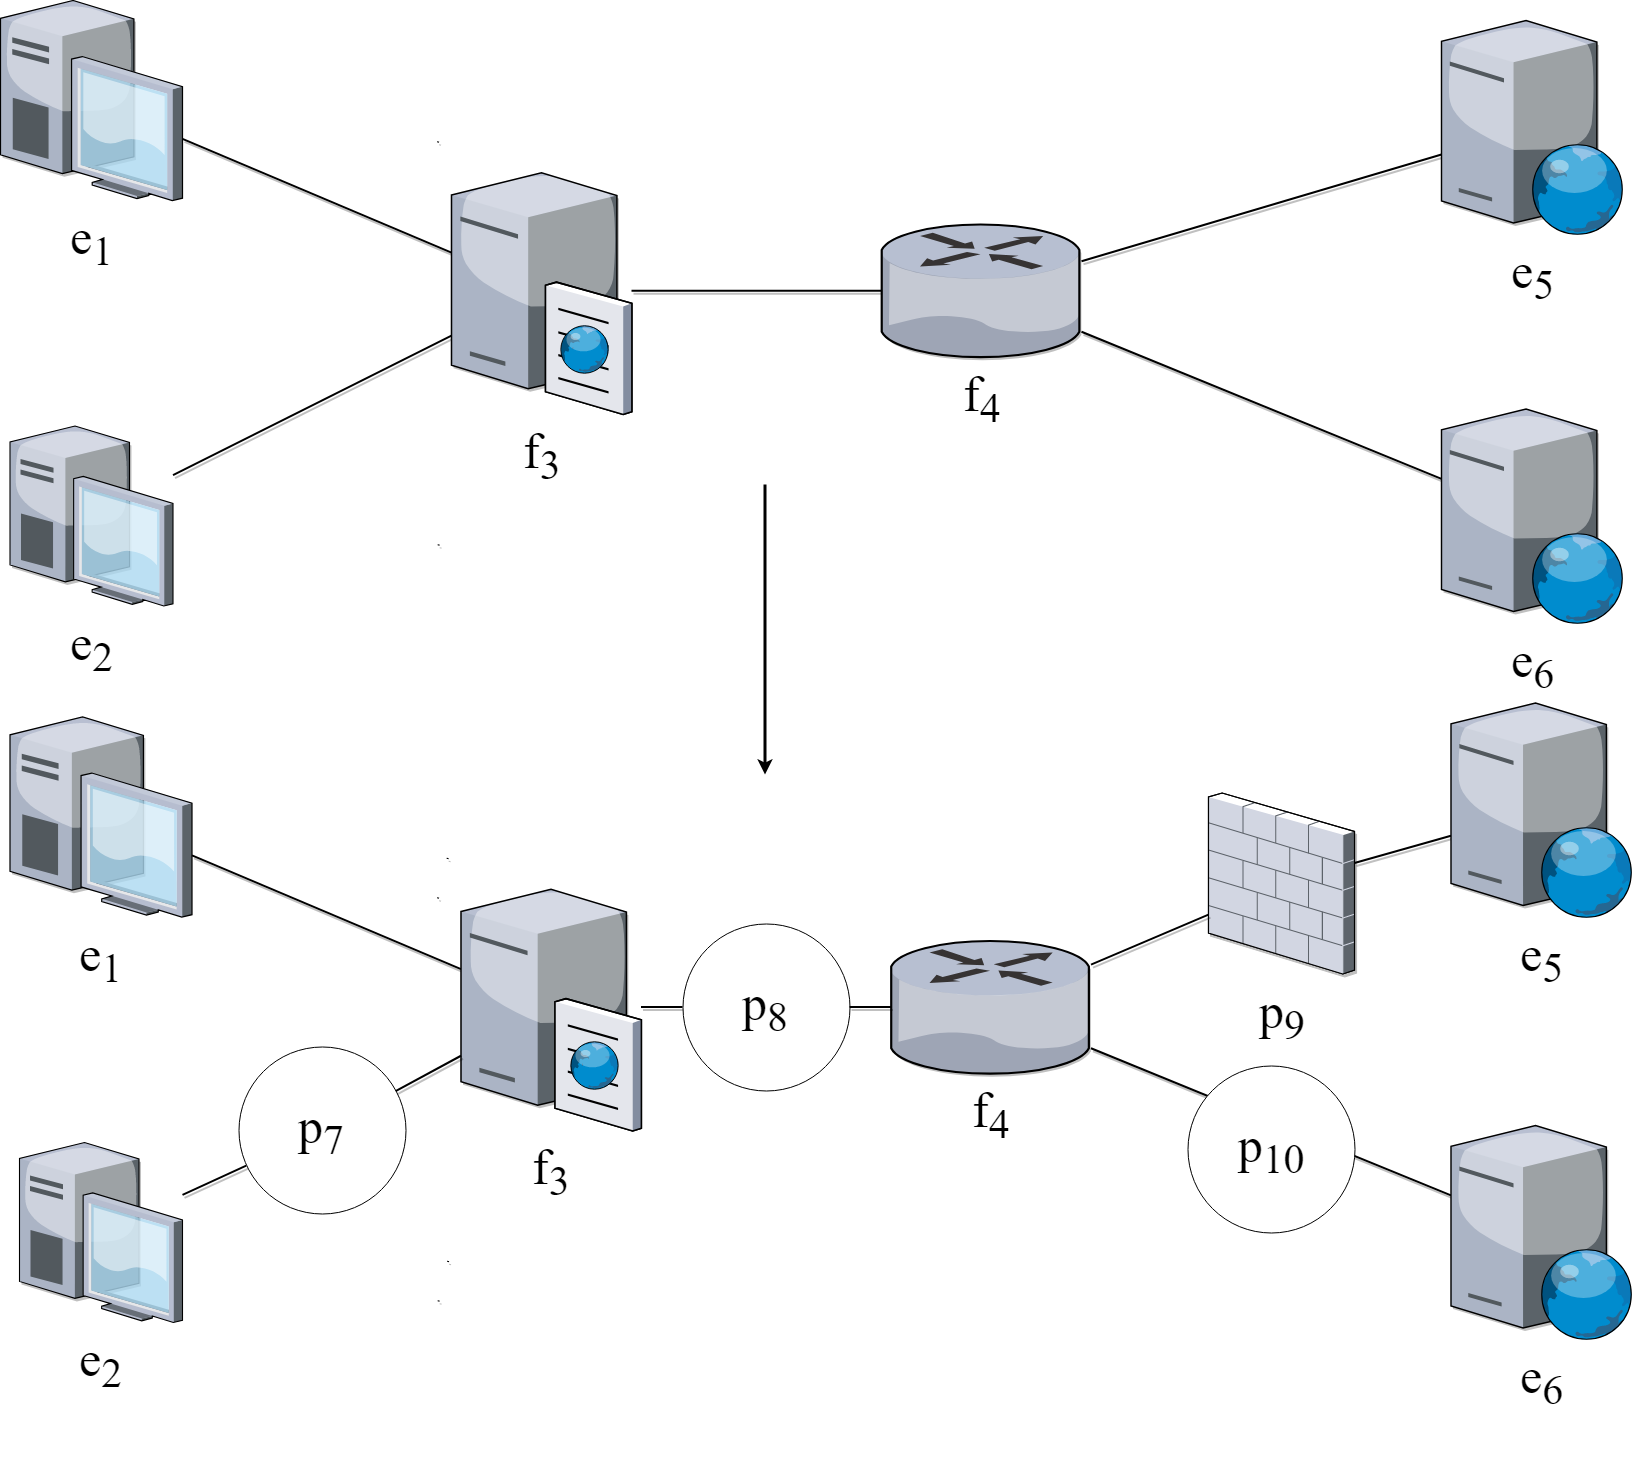
\includegraphics[width=0.4\textwidth]{images/stoa.png}}
	\caption{Automatic generation of an Allocation Graph}
	\label{fig:stoa}
\end{figure}

In this context, a consistent part of the thesis work has been dedicated to the definition of the hard constraints for the forwarding rules of the middle-boxes of the Allocation Graph. The exploited MaxSMT solver -- z3 -- would offer a tool, called \textit{quantifiers}, to express a set of nodes with a single variable and easily create forwarding rules, but it does not put any constraint which would allow to establish the minimum size of this set, with a consequent worsening of the performance the framework could reach. 

The problem which has been challenged, therefore, has been to identify the minimum set of nodes to which a packet can be sent, given a specific port from which it has been previously received, in order to reach the destination. This step has been fundamental to achieve good scalability for the methodology.

\subsection{Network Security Requirements}

The second input is represented by the \textit{Network Security Requirements}, hard constraints which must be enforced in the network to guarantee the required security level. The focus of the thesis was on \textit{connectivity} requirements between a pair of end points. In more details, they can be classified in two different types: 
\begin{enumerate}
\setlength\itemsep{-0.3em}
\item \textit{reachability property}, if a specific traffic flow must be allowed between a pair of end points;
\item \textit{isolation property}, if a specific traffic flow must be denied between a pair of end points.
\end{enumerate}
In this context, each traffic flow is identified by the source and destination IP addresses, the source and destination ports and the transport-level protocol.

In the definitions of the hard constraints representing the NSRs, which are not relaxable clauses because they are necessary conditions to fulfil, some of the aspects which have been considered are the possibility to define bidirectional requirements (e.g. a communication from an end point to another is allowed, while the opposite traffic flow is denied) and to define multiple requirements between the same pair of nodes (e.g. an endpoint can reach another at the destination port 80, while if it tries to contact the port 90 the packets must be blocked). This second example is represented in Figure \ref{fig:multiple03}, where a firewall allows only a specific traffic flow while blocking the others since it is in whitelisting mode.

\begin{figure}[tbh]
	\centerline{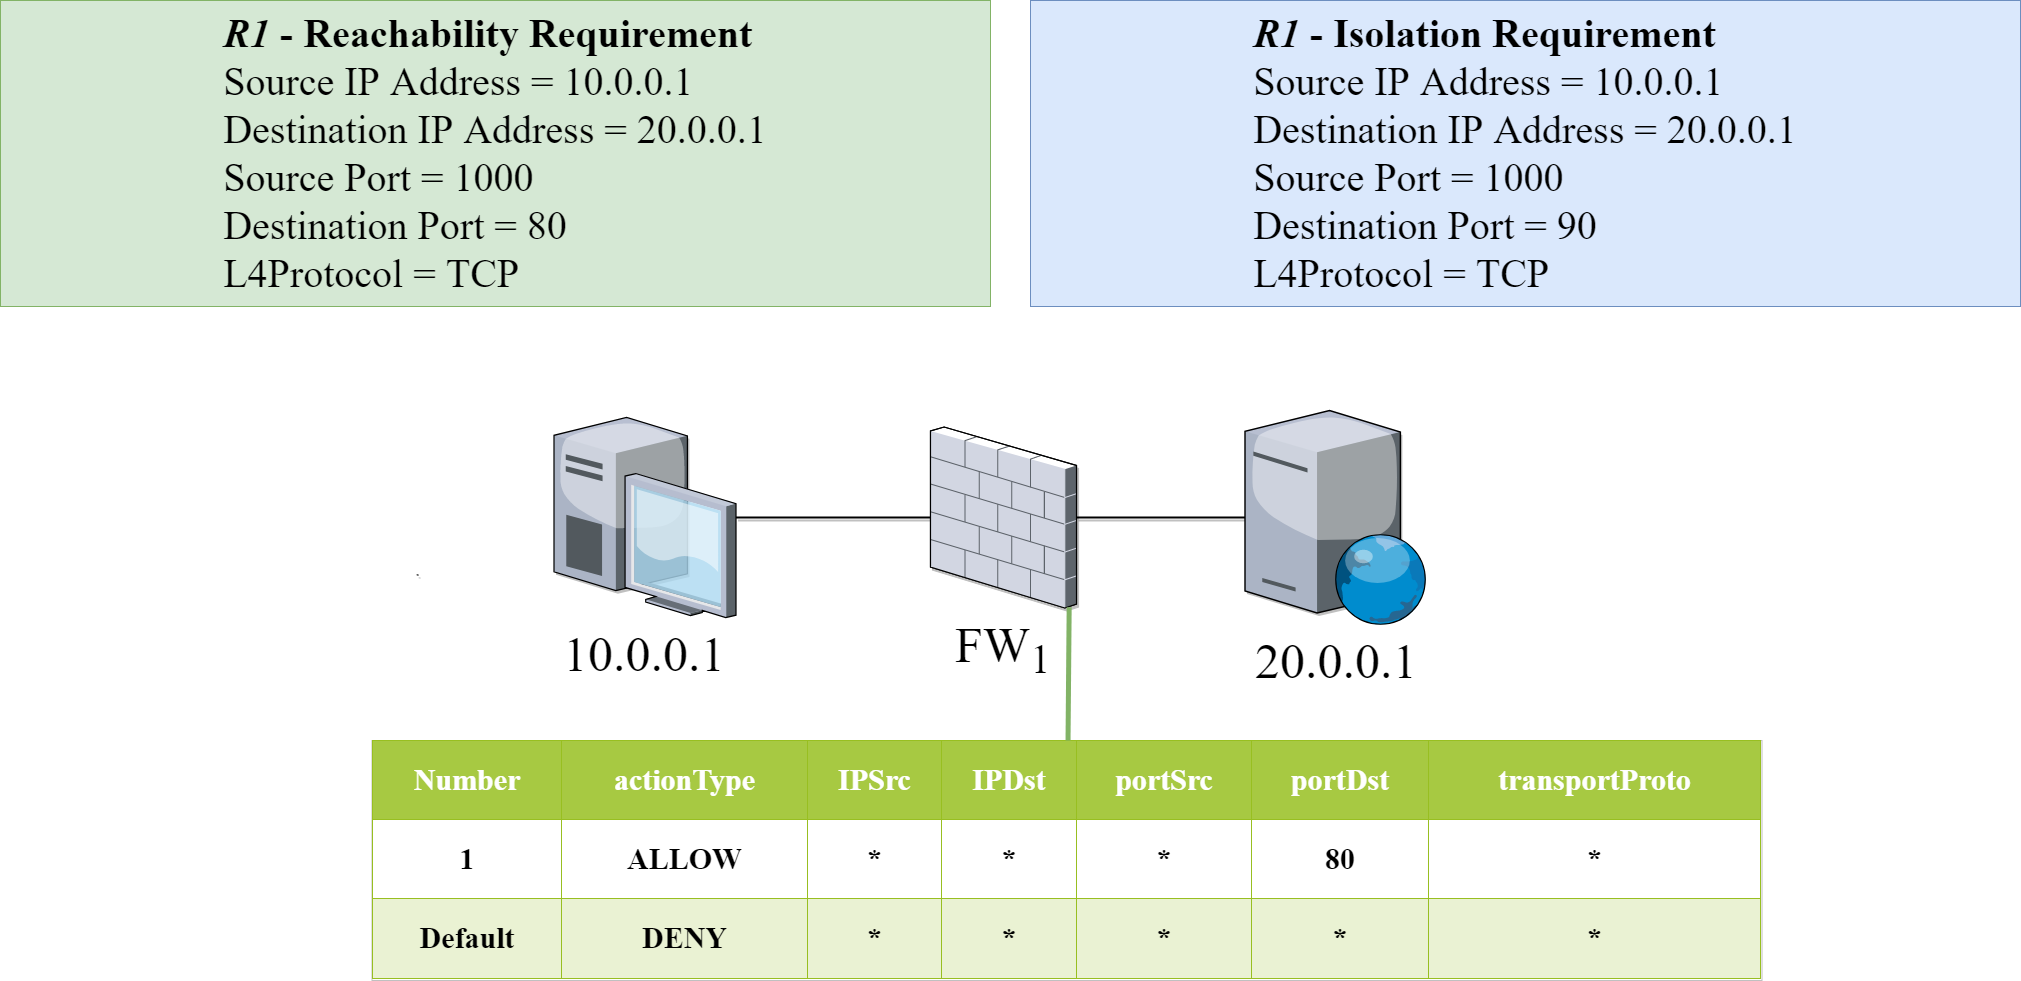
\includegraphics[width=0.5\textwidth]{images/multiple.png}}
	\caption{Example of NSRs between the same end points}
	\label{fig:multiple03}
\end{figure}

\subsection{Packet Filtering Firewalls}

A consistent part of the thesis work focused on defining the soft clauses to reach the optimal allocation of the firewalls in the Allocation Graph and the optimal auto-configuration of their Filtering Policies, that are made by a default action and a set of rules in order to decide if any packet must be forwarded or dropped. The actual objectives which have been modelled are:
\begin{enumerate}
	\setlength\itemsep{-0.3em}
	\item the minimization of the number of allocated firewalls, in order to reduce the resource consumption due to the deployment of the corresponding VNFs;
	\item the minimization of the number of rules for each Filtering Policy, in order to improve the efficiency of the filtering operations. 
\end{enumerate}

About the allocation objective, since the optimal solution would be that there is no need to instantiate VNFs for the packet filtering operation to reduce the resource consumption, then a set of clauses state that it is preferable that in each Allocation Place no firewall is allocated.%, as showed in Formula \ref{fm:soft_place}, where $c_{k}$ is the weight assigned to the corresponding soft clause.

%\begin{equation}  \label{fm:soft_place}
%\forall p_{k}, \; Soft(allocated(p_{k}) = false, \: c_{k1})
%\end{equation}

The critical component of the work has, instead, been related to the auto-configuration of the Filtering Policy rules. Starting from a simple approach where for each NSR the constraints for a corresponding placeholder rule are defined for each allocated firewall, to increase the efficiency of the methodology the thesis contributed to the developing of a number of pruning strategies to reduce the number of placeholder rules: for example, for a specific NSR, a rule is not needed when the default action already satisfies that requirements or when the corresponding traffic flow does not cross the firewall in exam.

A fundamental work has been made on the \textit{wildcards} feature, which allows to represent both an IP address and the netmask in a joint expression: for instance, the $10.0.0.\ast$ statement refers to the network 10.0.0.0/24. The same feature can be applied to transport-level ports and protocols. The idea has been to define the usage of wildcards for each component of the firewall rule as soft constraints, so that a single rule can satisfy contemporary more NSRs by defining larger IP addresses or port  ranges; this way, the solution space can be pruned before the execution of z3 optimizer engine, conspicuously improving the performance. 

Nevertheless, the usage of wildcards for each rule component is less primary than the absence itself of rule inside the firewall Filtering Policy. Consequently, after the definition of all the soft constraints, some time has been spent on the optimal tuning of their weights, so that the optimal solution could be achieved according to the proposed objectives in an efficient way.

\section{Implementation and Validation}

The implementation of the framework has been made by exploiting the Java language, since the z3 theorem prover offers Java APIs to formulate and solve the MaxSMT problem. The interaction with the framework can be made through REST APIs, so that it can be exploited by external tools as a component of a more complex architecture.

This implementation has been, finally, tested extensively in common network scenarios and it showed good scalability against the dimension of the Service Graph and the number of input security requirements. The charts illustrated by Figure \ref{fig:perf01} and Figure \ref{fig:perf02} present the result of a series of tests performed to compare the scalability of the framework implementation related respectively to the number of Allocation Places and Network Security Requirements; in particular, the MaxSAT instances have been solved on a machine with Intel i7-6700 CPU running at 3.40 GHz and
32GB of RAM. 

The first information that can be extracted from the two charts is that the computation time does not increase exponentially either with the number of Allocation Places or with the number of NSRs; this is a very important result, given the computational complexity of the MaxSMT problem. Moreover, the framework scales to Service Graphs of medium-big dimensions, with a high number of links and end points, providing the optimal solution to the presented problem.

It is then possible to notice that an increment of the NSRs number produces a computation time higher than the one produced by the same increment of the Allocation Places number. This result is motivated by the fact that the verification of each requirement must be performed in all the network, considering packets that flow across all the possible paths, whereas the constraints introduced by an additional Allocation Place only impact the traffic flow which crosses that node.

\begin{figure} [tbh]
	\centerline{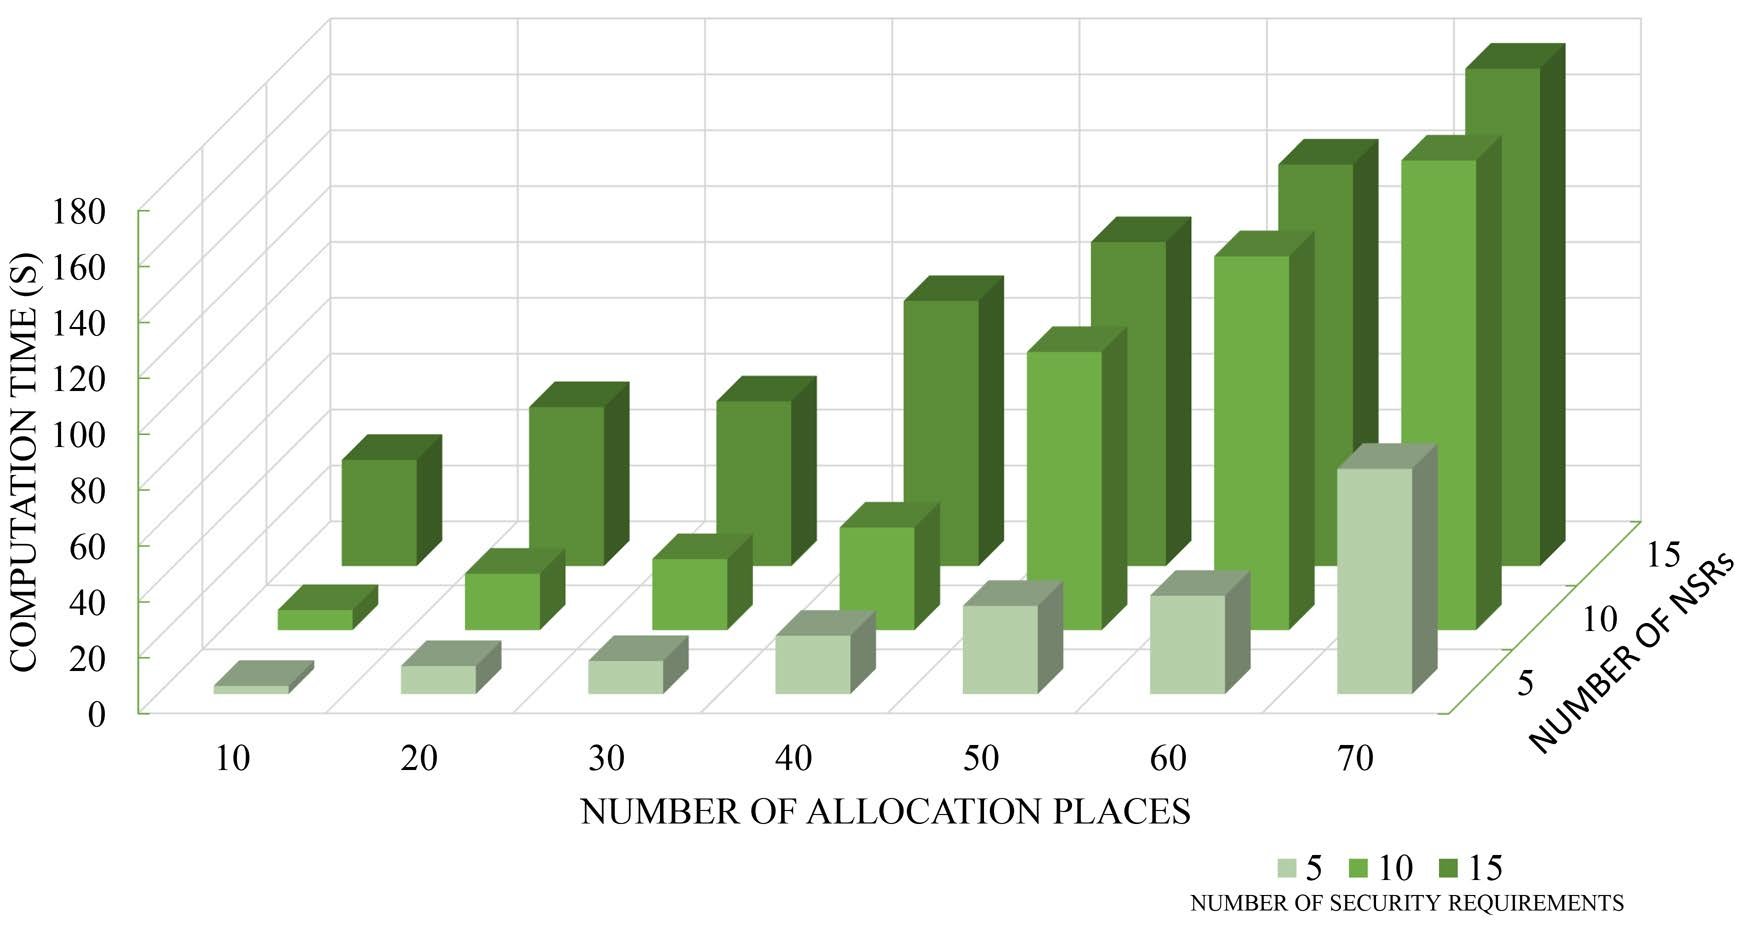
\includegraphics[width=0.5\textwidth]{images/scalability01.pdf}}
	\caption{Scalability tests on Allocation Places}
	\label{fig:perf01}
\end{figure}


\begin{figure} [tbh]
	\centerline{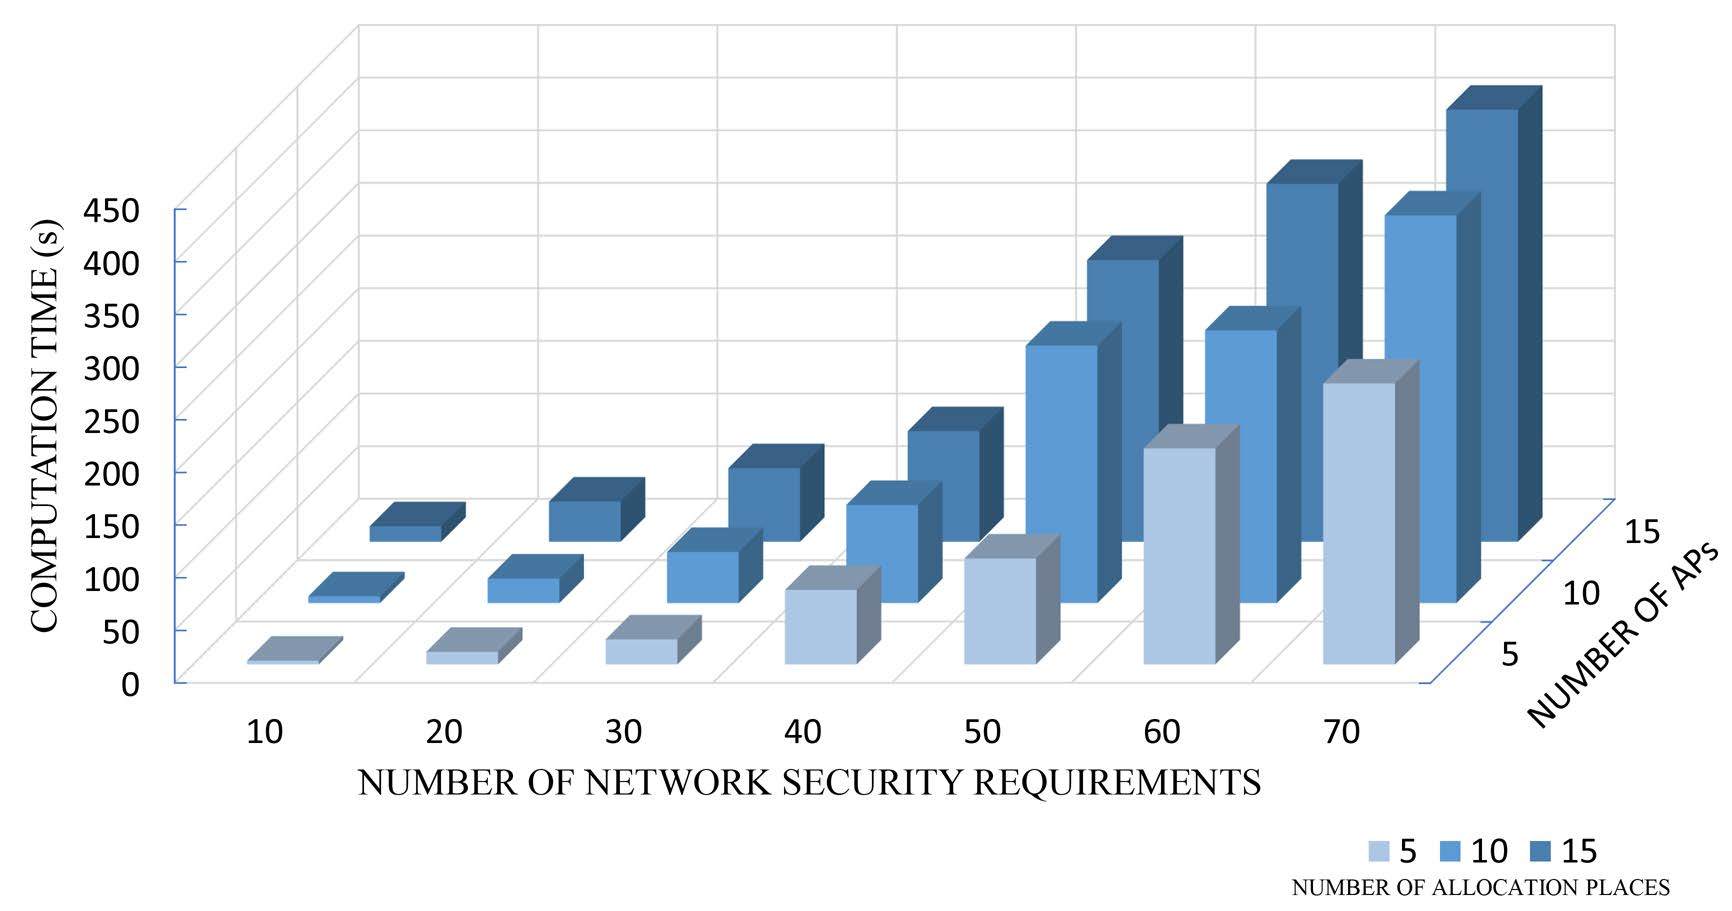
\includegraphics[width=0.5\textwidth]{images/scalability02.pdf}}
	\caption{Scalability tests on NSRs}
	\label{fig:perf02}
\end{figure}

\section{Conclusions and Future Work}
	 
This thesis demonstrates that the proposed approach is feasible and that it can provide a valid alternative in enforcing security functions to manual allocation and configuration of packet filtering firewalls, enabling low latency reaction to changes in security requirements. 

Furthermore, the approach has been developed to be compliant with future extensions such as the support of other NSFs in order to enrich its capabilities. Consequently, in the future the current methodology could be extended to the allocation and auto-configuration of other Network Security Functions, such as anti-spam filter, Web Application Firewall (WAF) and Intrusion Detection System (IDS). %, to further enrich the set of security requirements which can be specified by the user of the framework
Then, another possible future work is represented by the introduction of formal models for other network functions, such as the web cache, which the service designer can exploit to define the Service Graph.

%, on the other side definition of new Network Security Requirement types, which could consider additional features -- e.g. at application layer -- of the traffic flows to allow or to block. The goal would, in fact, be to further enrich the capabilities of the framework.

Finally, this thesis work represented the core content of a conference paper and a journal paper that will be submitted to IEEE/ACM Transactions on Networking in the next months.
	 
\end{document}

